% answers.tex —— 1993 年·上海卷 · 参考答案与详细解析片段
% 由 tools/generate_projects.py 依来源总账自 1993/1993_上海_试题.md + 1993/1993_上海_解析正文.md + 1993/1993_上海_答案要点.md 生成，勿手改（改源 MD 后重跑）


卷内第 1—10 题只列结果、第 11—20 题只列代号，第 21—26 题给出带分步给分的完整解答。以下按题整理，填空与选择题补出必要的推导，解答题以卷内解法为主线重述。

\gkpart{一、填空题（第 1—10 题）}

\begin{answer}
\gksolhead{1}{}

\textbf{题目}：

函数 $y=x^2-2x+3$ 的最小值是 \gkblank{}。

\Needspace{4\baselineskip}
\textbf{解析}

\Needspace{5\baselineskip}
配方得

\nopagebreak[4]
\[
y=x^2-2x+3=(x-1)^2+2.
\]

当 $x=1$ 时取最小值 $2$。

\gkanswer{答案：$2$。}

\end{answer}
\begin{answer}
\gksolhead{2}{}

\textbf{题目}：

函数 $y=\cos^2(\omega x)$（$\omega>0$）的最小正周期是 \gkblank{}。

\Needspace{4\baselineskip}
\textbf{解析}

\Needspace{5\baselineskip}
由降幂公式

\nopagebreak[4]
\[
\cos^2(\omega x)=\frac{1+\cos 2\omega x}{2},
\]

其最小正周期为 $\dfrac{2\pi}{2\omega}=\dfrac{\pi}{\omega}$。

\gkanswer{答案：$\dfrac{\pi}{\omega}$。}

\end{answer}
\begin{answer}
\gksolhead{3}{}

\textbf{题目}：

设 $z=\cos\dfrac{7\pi}{5}+i\sin\dfrac{7\pi}{5}$，$i$ 是虚数单位，则 $\bar z$ 的辐角主值是 \gkblank{}。

\Needspace{4\baselineskip}
\textbf{解析}

\Needspace{5\baselineskip}
$z$ 的模为 $1$，辐角为 $\dfrac{7\pi}{5}$，故 $\bar z$ 的辐角为 $-\dfrac{7\pi}{5}$。加上 $2\pi$ 化为辐角主值：

\nopagebreak[4]
\[
-\frac{7\pi}{5}+2\pi=\frac{3\pi}{5}.
\]

\gkanswer{答案：$\dfrac{3\pi}{5}$。}

\end{answer}
\begin{answer}
\gksolhead{4}{}

\textbf{题目}：

1 名老师和 4 名获奖同学排成一排照相留念，若老师不排在两端，则共有不同排法 \gkblank{} 种（结果用数值表示）。

\Needspace{4\baselineskip}
\textbf{解析}

\Needspace{5\baselineskip}
5 个位置中，老师不排两端，只能占中间 3 个位置之一；其余 4 名同学任意排列，有 $4!$ 种。故不同排法数为

\nopagebreak[4]
\[
3\times 4!=3\times 24=72.
\]

\gkanswer{答案：$72$。}

\end{answer}
\begin{answer}
\gksolhead{5}{}

\textbf{题目}：

函数 $y=\arccos x$（$-1\le x\le 0$）的反函数是 \gkblank{}。

\Needspace{4\baselineskip}
\textbf{解析}

\Needspace{5\baselineskip}
$y=\arccos x$ 在 $-1\le x\le 0$ 上的值域为 $\dfrac{\pi}{2}\le y\le\pi$。由 $y=\arccos x$ 得 $x=\cos y$，交换 $x$、$y$ 得反函数

\nopagebreak[4]
\[
y=\cos x,\qquad \frac{\pi}{2}\le x\le\pi.
\]

\gkanswer{答案：$y=\cos x$，$\dfrac{\pi}{2}\le x\le\pi$。}

\end{answer}
\begin{answer}
\gksolhead{6}{}

\textbf{题目}：

$P$ 点分 $\overline{AB}$ 所成的比是 $-3$，则 $B$ 点分 $\overline{AP}$ 所成的比是 \gkblank{}。

\Needspace{4\baselineskip}
\textbf{解析}

\Needspace{5\baselineskip}
设 $A$、$B$ 在数轴上对应 $0$、$1$，$P$ 对应 $t$。由 $P$ 分 $\overline{AB}$ 的比为 $-3$，即

\nopagebreak[4]
\[
\frac{AP}{PB}=\frac{t}{1-t}=-3,
\]

\Needspace{5\baselineskip}
解得 $t=\dfrac32$。于是 $B$ 分 $\overline{AP}$ 的比为

\nopagebreak[4]
\[
\frac{AB}{BP}=\frac{1}{\frac32-1}=2.
\]

\gkanswer{答案：$2$。}

\end{answer}
\begin{answer}
\gksolhead{7}{}

\textbf{题目}：

已知圆台的上、下底面半径分别是 $10\,\mathrm{cm}$ 和 $20\,\mathrm{cm}$，它的侧面展开后所得扇环的圆心角是 $180^\circ$，那么圆台的侧面积是 \gkblank{} $\mathrm{cm}^2$（结果中保留 $\pi$）。

\Needspace{4\baselineskip}
\textbf{解析}

\Needspace{5\baselineskip}
设圆台上、下底面半径为 $r=10$、$R=20$，母线长为 $l$。侧面展开所得扇环的圆心角为 $180^\circ=\pi$，而扇环圆心角等于 $\dfrac{2\pi(R-r)}{l}$，故

\nopagebreak[4]
\[
\pi=\frac{2\pi(20-10)}{l},\qquad l=20.
\]

\Needspace{5\baselineskip}
侧面积为

\nopagebreak[4]
\[
S_{\text{侧}}=\pi(R+r)l=\pi(20+10)\times 20=600\pi.
\]

\gkanswer{答案：$600\pi$。}

\end{answer}
\begin{answer}
\gksolhead{8}{}

\textbf{题目}：

已知等比数列 $\{a_n\}$（$a_n\in\mathbb{R}$），$a_1+a_2=9$，$a_1\cdot a_2\cdot a_3=27$，且 $S_n=a_1+a_2+\cdots+a_n$（$n=1,2,\ldots$），则 $\lim\limits_{n\to\infty}S_n=$ \gkblank{}。

\Needspace{4\baselineskip}
\textbf{解析}

\Needspace{5\baselineskip}
设公比为 $q$。由 $a_1+a_2=9$ 得 $a_1(1+q)=9$；由 $a_1a_2a_3=27$ 得 $(a_1q)^3=27$，即 $a_1q=3$。两式相减得 $a_1=6$，从而 $q=\dfrac12$。于是

\nopagebreak[4]
\[
\lim_{n\to\infty}S_n=\frac{a_1}{1-q}=\frac{6}{1-\frac12}=12.
\]

\gkanswer{答案：$12$。}

\end{answer}
\begin{answer}
\gksolhead{9}{}

\textbf{题目}：

在极坐标系中，过点 $M\left(2,\dfrac{\pi}{2}\right)$ 且平行于极轴的直线的极坐标方程是 \gkblank{}。

\Needspace{4\baselineskip}
\textbf{解析}

\Needspace{5\baselineskip}
点 $M\left(2,\dfrac{\pi}{2}\right)$ 的直角坐标为 $(0,2)$。过该点且平行于极轴（即 $x$ 轴）的直线为 $y=2$，化为极坐标方程即

\nopagebreak[4]
\[
\rho\sin\theta=2.
\]

\gkanswer{答案：$\rho\sin\theta=2$。}

\end{answer}
\begin{answer}
\gksolhead{10}{}

\textbf{题目}：

如图，正方体 $ABCD-A_1B_1C_1D_1$ 中，过顶点 $B$、$D$、$C_1$ 作截面，则二面角 $B\text{-}DC_1\text{-}C$ 的大小是 \gkblank{}（用反三角函数表示）。
\nopagebreak[4]
\begin{center}% 依固定扫描页重绘；仅示意正方体的拓扑、顶点标号与过 B、D、C_1 的截面，不按比例。
% 投影坐标只为作图，不表示题设给出坐标或边长。下底面为 ABCD，上底面为 A_1B_1C_1D_1。
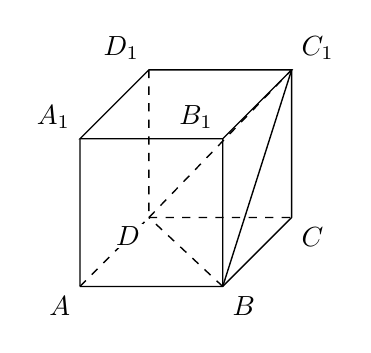
\begin{tikzpicture}[line width=.5pt,scale=1.25]
  \coordinate (A1) at (0,1.7);
  \coordinate (B1) at (1.45,1.7);
  \coordinate (C1) at (2.15,2.4);
  \coordinate (D1) at (.7,2.4);
  \coordinate (A) at (0,.2);
  \coordinate (B) at (1.45,.2);
  \coordinate (C) at (2.15,.9);
  \coordinate (D) at (.7,.9);
  % 上底面、可见外棱与隐藏外棱。
  \draw (A1)--(B1)--(C1)--(D1)--cycle;
  \draw (A1)--(A) (B1)--(B) (C1)--(C) (A)--(B)--(C);
  \draw[dashed] (D1)--(D) (A)--(D) (D)--(C);
  % 截面 BDC_1：BD 位于下底面、DC_1 位于背面，按投影用虚线表示。
  \draw (B)--(C1);
  \draw[dashed] (B)--(D) (D)--(C1);
  \node[above left] at (A1) {$A_1$};
  \node[above left] at (B1) {$B_1$};
  \node[above right] at (C1) {$C_1$};
  \node[above left] at (D1) {$D_1$};
  \node[below left] at (A) {$A$};
  \node[below right] at (B) {$B$};
  \node[below right] at (C) {$C$};
  \node[fill=white,inner sep=1pt,below left=2pt] at (D) {$D$};
\end{tikzpicture}
\end{center}
\nopagebreak[4]
\Needspace{4\baselineskip}
\textbf{解析}

\Needspace{5\baselineskip}
设立方体棱长为 $1$，取坐标

\nopagebreak[4]
\[
A(0,0,0),\quad B(1,0,0),\quad C(1,1,0),\quad D(0,1,0),\quad C_1(1,1,1).
\]

\Needspace{5\baselineskip}
平面 $BDC_1$ 内两向量

\nopagebreak[4]
\[
\overrightarrow{DB}=(1,-1,0),\qquad \overrightarrow{DC_1}=(1,0,1),
\]

\Needspace{5\baselineskip}
其法向量可取

\nopagebreak[4]
\[
\vec n_1=\overrightarrow{DB}\times\overrightarrow{DC_1}=(-1,-1,1).
\]

\Needspace{5\baselineskip}
平面 $DCC_1$ 即 $y=1$，法向量可取 $\vec n_2=(0,1,0)$。故两平面夹角 $\theta$ 满足

\nopagebreak[4]
\[
\cos\theta=\frac{|\vec n_1\cdot\vec n_2|}{|\vec n_1||\vec n_2|}
=\frac{1}{\sqrt3}=\frac{\sqrt3}{3}.
\]

因此二面角 $B\text{-}DC_1\text{-}C$ 的大小为 $\arccos\dfrac{\sqrt3}{3}$。

\gkanswer{答案：$\arccos\dfrac{\sqrt3}{3}$。}

\end{answer}
\gkpart{二、选择题（第 11—20 题）}

\begin{answer}
\gksolhead{11}{}

\textbf{题目}：

函数 $y=x+a$ 与 $y=\log_a x$ 的图象可能是（　）。

（A）图 A；（B）图 B；（C）图 C；（D）图 D。
\nopagebreak[4]
\begin{center}% 依固定扫描页重绘；四个面板只示意直线 y=x+a 的截距位置与曲线 y=log_a x 的增减方向，不按比例。
% 只有 (C) 用同一个 0<a<1 同时满足两函数的图象特征。
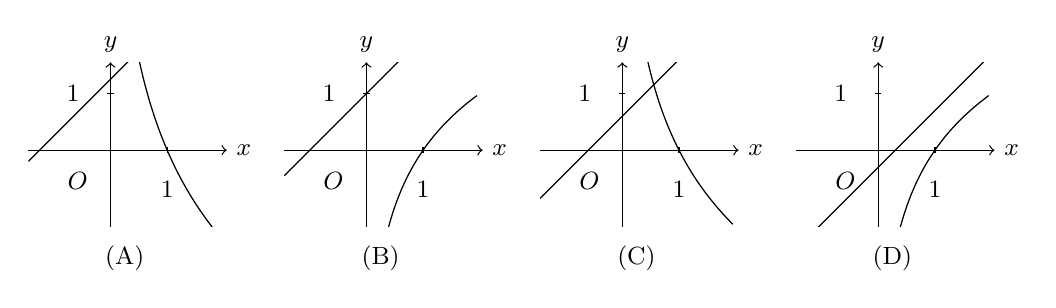
\begin{tikzpicture}[line width=.45pt,x=.72cm,y=.72cm,font=\small]
  \foreach \panel/\shift/\linea/\loga in {A/0/1.25/.65,B/3.25/1/2,C/6.5/.6/.6,D/9.75/-.3/2}{
    \begin{scope}[xshift=\shift cm]
      \begin{scope}
        \clip (-1.45,-1.35) rectangle (2.05,1.55);
        \draw[domain=.34:1.95,samples=70,smooth] plot (\x,{ln(\x)/ln(\loga)});
        \draw[domain=-1.45:2.05,samples=2] plot (\x,{\x+\linea});
      \end{scope}
      \draw[->] (-1.45,0)--(2.05,0) node[right] {$x$};
      \draw[->] (0,-1.35)--(0,1.55) node[above] {$y$};
      \draw (-.055,1)--(.055,1);
      \node[left=10pt,inner sep=1pt] at (0,1) {$1$};
      \draw (1,-.055)--(1,.055);
      \node[below=10pt,inner sep=1pt] at (1,0) {$1$};
      \node[below left=7pt,inner sep=1pt] at (0,0) {$O$};
      \node at (.25,-1.9) {(\panel)};
    \end{scope}
  }
\end{tikzpicture}
\end{center}
\nopagebreak[4]
\Needspace{4\baselineskip}
\textbf{解析}

直线 $y=x+a$ 的斜率为 $1$，纵截距为 $a$，横截距为 $-a$；曲线 $y=\log_a x$ 过点 $(1,0)$，当 $a>1$ 时递增，当 $0<a<1$ 时递减。逐幅检验：

（A）直线纵截距大于 $1$，要求 $a>1$，但曲线递减，要求 $0<a<1$，矛盾；

（B）直线纵截距等于 $1$，即 $a=1$，而对数函数的底数要求 $a\ne1$，矛盾；

（C）直线纵截距在 $(0,1)$ 内，即 $0<a<1$，曲线递减，一致；

（D）直线纵截距为负，即 $a<0$，与 $a>0$ 矛盾。

故选（C）。

\gkanswer{答案：C。}

\end{answer}
\begin{answer}
\gksolhead{12}{}

\textbf{题目}：

$(x-1)^9$ 按 $x$ 降幂排列的展开式中，系数最大的项是（　）。

（A）第 4 项和第 5 项；（B）第 5 项；（C）第 5 项和第 6 项；（D）第 6 项。

\Needspace{4\baselineskip}
\textbf{解析}

\Needspace{5\baselineskip}
展开式的第 $k+1$ 项为

\nopagebreak[4]
\[
T_{k+1}=\mathrm C_9^k x^{9-k}(-1)^k.
\]

\Needspace{5\baselineskip}
各项系数依次为

\nopagebreak[4]
\[
1,\ -9,\ 36,\ -84,\ 126,\ -126,\ 84,\ -36,\ 9,\ -1.
\]

按有符号系数比较，最大者为 $126$，是第 $5$ 项。故选（B）。

\gkanswer{答案：B。}

\end{answer}
\begin{answer}
\gksolhead{13}{}

\textbf{题目}：

在区间 $(0,+\infty)$ 上为增函数的是（　）。

（A）$y=\operatorname{arcctg}x$；（B）$y=\log_{1/2}x$；（C）$y=-2^x$；（D）$y=x^{1/3}$。

\Needspace{4\baselineskip}
\textbf{解析}

在 $(0,+\infty)$ 上：$y=\operatorname{arcctg}x$ 递减；$y=\log_{1/2}x$ 递减；$y=-2^x$ 递减；$y=x^{1/3}$ 递增。故选（D）。

\gkanswer{答案：D。}

\end{answer}
\begin{answer}
\gksolhead{14}{}

\textbf{题目}：

下列不等式中正确的是（　）。

（A）$\arcsin\left(-\dfrac14\right)<\arcsin\left(-\dfrac13\right)$；

（B）$\arccos\left(-\dfrac14\right)<\arccos\dfrac13$；

（C）$\operatorname{arctg}\dfrac14<\arcsin\dfrac14$；

（D）$\operatorname{arcctg}\dfrac13<\operatorname{arctg}\dfrac13$。

\Needspace{4\baselineskip}
\textbf{解析}

（A）$\arcsin x$ 在 $[-1,1]$ 上递增，而 $-\dfrac14>-\dfrac13$，故 $\arcsin\left(-\dfrac14\right)>\arcsin\left(-\dfrac13\right)$，错；

（B）$\arccos x$ 在 $[-1,1]$ 上递减，而 $-\dfrac14<\dfrac13$，故 $\arccos\left(-\dfrac14\right)>\arccos\dfrac13$，错；

（C）当 $0<t<1$ 时，$\operatorname{tg}(\arcsin t)=\dfrac{t}{\sqrt{1-t^2}}>t=\operatorname{tg}(\operatorname{arctg}t)$，且两角均在 $\left(0,\dfrac{\pi}{2}\right)$ 内，故 $\arcsin t>\operatorname{arctg}t$。取 $t=\dfrac14$ 即得 $\operatorname{arctg}\dfrac14<\arcsin\dfrac14$，正确；

（D）$\operatorname{arcctg}\dfrac13=\operatorname{arctg}3>\operatorname{arctg}\dfrac13$，错。

故选（C）。

\gkanswer{答案：C。}

\end{answer}
\begin{answer}
\gksolhead{15}{}

\textbf{题目}：

动点 $P$ 到直线 $x+4=0$ 的距离减去它到点 $M(2,0)$ 的距离之差等于 2，则点 $P$ 的轨迹是（　）。

（A）直线；（B）椭圆；（C）双曲线；（D）抛物线。

\Needspace{4\baselineskip}
\textbf{解析}

\Needspace{5\baselineskip}
设 $P(x,y)$。到直线 $x+4=0$ 的距离为 $|x+4|$，到 $M(2,0)$ 的距离为 $\sqrt{(x-2)^2+y^2}$。由题意

\nopagebreak[4]
\[
|x+4|-\sqrt{(x-2)^2+y^2}=2.
\]

\Needspace{5\baselineskip}
轨迹在直线右侧，取 $x+4>0$，则

\nopagebreak[4]
\[
\sqrt{(x-2)^2+y^2}=x+2.
\]

\Needspace{5\baselineskip}
两边平方得

\nopagebreak[4]
\[
(x-2)^2+y^2=(x+2)^2 \quad\Longrightarrow\quad y^2=8x.
\]

这是抛物线，故点 $P$ 的轨迹是抛物线。选（D）。

\gkanswer{答案：D。}

\end{answer}
\begin{answer}
\gksolhead{16}{}

\textbf{题目}：

设有三个命题：

甲、底面是平行四边形的四棱柱是平行六面体；

乙、底面是矩形的平行六面体是长方体；

丙、直四棱柱是直平行六面体。

以上命题中真命题的个数是（　）。

（A）0；（B）1；（C）2；（D）3。

\Needspace{4\baselineskip}
\textbf{解析}

甲：底面为平行四边形的四棱柱，其各侧面均为平行四边形，是平行六面体，真。

乙：底面为矩形的平行六面体，侧棱仍可倾斜，不一定是直棱柱，因而不一定是长方体，假。

丙：直四棱柱只保证侧棱垂直于底面；若底面是一般四边形而非平行四边形，它就不是平行六面体，假。

真命题只有 $1$ 个。故选（B）。

\gkanswer{答案：B。}

\end{answer}
\begin{answer}
\gksolhead{17}{}

\textbf{题目}：

在直角坐标系中平移坐标轴，把原点 $O(0,0)$ 移到 $O'(2,-5)$，点 $A$ 在新坐标系中的坐标为 $(-3,7)$，则点 $A$ 在原坐标系中的坐标是（　）。

（A）$(-1,2)$；（B）$(1,-2)$；（C）$(-5,12)$；（D）$(5,-12)$。

\Needspace{4\baselineskip}
\textbf{解析}

\Needspace{5\baselineskip}
坐标轴平移后，新坐标与旧坐标的关系为

\nopagebreak[4]
\[
x'=x-2,\qquad y'=y+5.
\]

\Needspace{5\baselineskip}
已知 $A$ 的新坐标 $(x',y')=(-3,7)$，故

\nopagebreak[4]
\[
x=x'+2=-1,\qquad y=y'-5=2.
\]

即 $A(-1,2)$。故选（A）。

\gkanswer{答案：A。}

\end{answer}
\begin{answer}
\gksolhead{18}{}

\textbf{题目}：

设 $a$、$b$ 是两条异面直线。在下列命题中正确的是（　）。

（A）有且仅有一条直线与 $a$、$b$ 都垂直；

（B）有一平面与 $a$、$b$ 都垂直；

（C）过直线 $a$ 有且仅有一平面与 $b$ 平行；

（D）过空间中任一点必可作一条直线与 $a$、$b$ 都相交。

\Needspace{4\baselineskip}
\textbf{解析}

（A）与两条异面直线都垂直的直线有无数条，它们的方向均为两直线方向向量的叉积方向，只是位置不同，假；

（B）若一平面与 $a$、$b$ 都垂直，则 $a$、$b$ 都垂直于该平面，从而 $a\parallel b$，与异面矛盾，假；

（C）过直线 $a$ 上一点作直线 $b'\parallel b$，$a$ 与 $b'$ 确定的平面即为过 $a$ 且平行于 $b$ 的平面；这样的平面唯一，真；

（D）过空间中任一点不一定能作一条直线同时与两条异面直线相交，假。

故选（C）。

\gkanswer{答案：C。}

\end{answer}
\begin{answer}
\gksolhead{19}{}

\textbf{题目}：

函数 $y=\cos\left(2x+\dfrac{\pi}{2}\right)$ 的图象的一条对称轴方程是（　）。

（A）$x=-\dfrac{\pi}{2}$；（B）$x=-\dfrac{\pi}{4}$；（C）$x=\dfrac{\pi}{8}$；（D）$x=\pi$。

\Needspace{4\baselineskip}
\textbf{解析}

\nopagebreak[4]
\[
y=\cos\left(2x+\frac{\pi}{2}\right)=-\sin 2x.
\]

\Needspace{5\baselineskip}
其对称轴是使 $\sin 2x=\pm1$ 的直线：

\nopagebreak[4]
\[
2x=\frac{\pi}{2}+k\pi,\qquad x=\frac{\pi}{4}+\frac{k\pi}{2}\quad(k\in\mathbb Z).
\]

取 $k=-1$ 得 $x=-\dfrac{\pi}{4}$。故选（B）。

\gkanswer{答案：B。}

\end{answer}
\begin{answer}
\gksolhead{20}{}

\textbf{题目}：

“$a+b>2c$”的一个充分条件是（　）。

（A）$a>c$ 或 $b>c$；（B）$a>c$ 且 $b<c$；（C）$a>c$ 且 $b>c$；（D）$a>c$ 或 $b<c$。

\Needspace{4\baselineskip}
\textbf{解析}

\Needspace{5\baselineskip}
若 $a>c$ 且 $b>c$，则

\nopagebreak[4]
\[
a+b>c+c=2c.
\]

故 $a>c$ 且 $b>c$ 是 $a+b>2c$ 的充分条件。其余选项均不能保证：如（A）（D）只要求一个大于 $c$，（B）中 $b<c$ 可能使 $a+b\le 2c$。故选（C）。

\gkanswer{答案：C。}

\end{answer}
\gkpart{三、解答题（第 21—23 题）}

\begin{answer}
\gksolhead{21}{}

\textbf{题目}：

（本题满分 12 分）

已知角 $\alpha$ 的顶点与直角坐标系的原点重合，始边在 $x$ 轴的正半轴上，终边经过点 $P(-1,2)$，求 $\sin\left(2\alpha+\frac{2\pi}{3}\right)$ 的值。

\Needspace{4\baselineskip}
\textbf{解析}

\Needspace{5\baselineskip}
由 $P(-1,2)$ 得

\nopagebreak[4]
\[
r=|OP|=\sqrt{(-1)^2+2^2}=\sqrt5,
\]

\Needspace{5\baselineskip}
故

\nopagebreak[4]
\[
\sin\alpha=\frac{2}{\sqrt5},\qquad \cos\alpha=-\frac{1}{\sqrt5}.
\]

\Needspace{5\baselineskip}
于是

\nopagebreak[4]
\[
\sin 2\alpha=2\sin\alpha\cos\alpha=-\frac45,
\]

\nopagebreak[4]
\[
\cos 2\alpha=1-2\sin^2\alpha=1-\frac85=-\frac35.
\]

\Needspace{5\baselineskip}
所以

\nopagebreak[4]
\[
\begin{aligned}
\sin\left(2\alpha+\frac{2\pi}{3}\right)
&=\sin 2\alpha\cos\frac{2\pi}{3}+\cos 2\alpha\sin\frac{2\pi}{3}\\
&=\left(-\frac45\right)\left(-\frac12\right)
+\left(-\frac35\right)\frac{\sqrt3}{2}\\
&=\frac25-\frac{3\sqrt3}{10}
=\frac{4-3\sqrt3}{10}.
\end{aligned}
\]

\gkanswer{答案：$\dfrac{4-3\sqrt3}{10}$。}

\end{answer}
\begin{answer}
\gksolhead{22}{}

\textbf{题目}：

（本题满分 12 分）

已知 $z=\dfrac{a-i}{1-i}$，其中 $i$ 为虚数单位，$a>0$，复数 $w=z(z+i)$ 的虚部减去它的实部所得的差等于 $\dfrac32$，求复数 $w$ 的模。

\Needspace{4\baselineskip}
\textbf{解析}

\Needspace{5\baselineskip}
先化简 $w$：

\nopagebreak[4]
\[
\begin{aligned}
w&=z(z+i)=\frac{a-i}{1-i}\left(\frac{a-i}{1-i}+i\right)\\
&=\frac{a-i}{1-i}\cdot\frac{a-i+i(1-i)}{1-i}\\
&=\frac{(a-i)(a+1)}{(1-i)^2}.
\end{aligned}
\]

\Needspace{5\baselineskip}
由 $(1-i)^2=-2i$，得

\nopagebreak[4]
\[
w=\frac{(a-i)(a+1)}{-2i}
=\frac{a+1}{2}(1+ai).
\]

\Needspace{5\baselineskip}
其实部为 $\dfrac{a+1}{2}$，虚部为 $\dfrac{a(a+1)}{2}$。由题意虚部减实部等于 $\dfrac32$：

\nopagebreak[4]
\[
\frac{a(a+1)}{2}-\frac{a+1}{2}=\frac32,
\]

\Needspace{5\baselineskip}
即

\nopagebreak[4]
\[
\frac{(a+1)(a-1)}{2}=\frac32,\qquad a^2-1=3,\qquad a^2=4.
\]

\Needspace{5\baselineskip}
因 $a>0$，故 $a=2$。于是

\nopagebreak[4]
\[
w=\frac32(1+2i)=\frac32+3i,
\]

\nopagebreak[4]
\[
|w|=\sqrt{\left(\frac32\right)^2+3^2}
=\sqrt{\frac94+9}
=\frac{3\sqrt5}{2}.
\]

\gkanswer{答案：$|w|=\dfrac{3\sqrt5}{2}$。}

\end{answer}
\begin{answer}
\gksolhead{23}{}

\textbf{题目}：

（本题满分 12 分）

抛物线 $y=-\dfrac{x^2}{2}$ 与过点 $M(0,-1)$ 的直线 $l$ 相交于 $A$、$B$ 两点，$O$ 为坐标原点。若直线 $OA$ 与 $OB$ 的斜率之和为 1，求直线 $l$ 的方程。

\Needspace{4\baselineskip}
\textbf{解析}

\Needspace{5\baselineskip}
设 $A(x_1,y_1)$、$B(x_2,y_2)$。直线 $l$ 过 $M(0,-1)$，设其方程为

\nopagebreak[4]
\[
y=kx-1.
\]

\Needspace{5\baselineskip}
代入抛物线方程 $y=-\dfrac{x^2}{2}$，得

\nopagebreak[4]
\[
-\frac{x^2}{2}=kx-1 \quad\Longrightarrow\quad x^2+2kx-2=0.
\]

\Needspace{5\baselineskip}
由韦达定理

\nopagebreak[4]
\[
x_1+x_2=-2k,\qquad x_1x_2=-2.
\]

\Needspace{5\baselineskip}
直线 $OA$、$OB$ 的斜率之和为

\nopagebreak[4]
\[
k_{OA}+k_{OB}=\frac{y_1}{x_1}+\frac{y_2}{x_2}.
\]

\Needspace{5\baselineskip}
因 $y_i=-\dfrac{x_i^2}{2}$，故 $\dfrac{y_i}{x_i}=-\dfrac{x_i}{2}$，于是

\nopagebreak[4]
\[
k_{OA}+k_{OB}=-\frac{x_1+x_2}{2}
=-\frac{-2k}{2}=k.
\]

\Needspace{5\baselineskip}
由题意 $k=1$。因此直线 $l$ 的方程为

\nopagebreak[4]
\[
y=x-1.
\]

\gkanswer{答案：直线 $l$ 的方程为 $y=x-1$。}

\end{answer}
\gkpart{四、解答题（第 24—26 题）}

\begin{answer}
\gksolhead{24}{}

\textbf{题目}：

（本题满分 16 分）本题共有 3 小题，第 1 小题满分 5 分，第 2 小题满分 5 分，第 3 小题满分 6 分。

如图，已知二面角 $\alpha\text{-}PQ\text{-}\beta$ 为 $60^\circ$，点 $A$ 和点 $B$ 分别在平面 $\alpha$ 和平面 $\beta$ 上，点 $C$ 在棱 $PQ$ 上，$\angle ACP=\angle BCP=30^\circ$，$CA=CB=a$。

（1）求证 $AB\perp PQ$；

（2）求点 $B$ 到平面 $\alpha$ 的距离；

（3）设 $R$ 是线段 $OA$ 上的一点，直线 $BR$ 与平面 $\alpha$ 所成角的大小为 $45^\circ$，求线段 $CR$ 的长度。
\nopagebreak[4]
\begin{center}% 依固定扫描页重绘；两平面以平行四边形示意，交棱为 PQ，A 在平面 α 内，B 在平面 β 内，C 在 PQ 上。
% 面片与投影仅为拓扑示意，不按比例；不编码题面未给出的长度、角度、垂足或点 O 的定义。
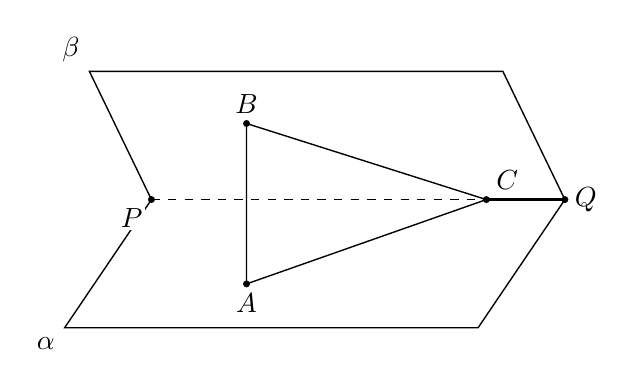
\begin{tikzpicture}[line width=.5pt,scale=1.05]
  \coordinate (P) at (0,0);
  \coordinate (Q) at (5,0);
  \coordinate (BtL) at (-.75,1.55);
  \coordinate (BtR) at (4.25,1.55);
  \coordinate (AlL) at (-1.05,-1.55);
  \coordinate (AlR) at (3.95,-1.55);
  \coordinate (A) at (1.15,-1.02);
  \coordinate (B) at (1.15,.92);
  \coordinate (C) at (4.05,0);
  % 两个平面以平行四边形作投影边界，共用棱 PQ。
  \draw (P)--(BtL)--(BtR)--(Q);
  \draw (P)--(AlL)--(AlR)--(Q);
  \draw[dashed] (P)--(C);
  \draw[thick] (C)--(Q);
  % 原图中的三角形 ABC 与交棱关系。
  \draw (A)--(B)--(C)--cycle;
  \fill (P) circle (1.2pt) (Q) circle (1.2pt) (A) circle (1.2pt)
    (B) circle (1.2pt) (C) circle (1.2pt);
  \node[fill=white,inner sep=1pt,below left=2pt] at (P) {$P$};
  \node[right] at (Q) {$Q$};
  \node[below] at (A) {$A$};
  \node[above] at (B) {$B$};
  \node[above right] at (C) {$C$};
  \node[above left] at (BtL) {$\beta$};
  \node[below left] at (AlL) {$\alpha$};
\end{tikzpicture}
\end{center}
\nopagebreak[4]
\Needspace{4\baselineskip}
\textbf{解析}

题面第（3）问印作“线段 $OA$ 上的一点”，但题面与图中均未定义点 $O$；卷内解答按 $R$ 在线段 $CA$ 上计算。以下按 $CA$ 理解，题面文字照录于试题文件。

（1）在平面 $\beta$ 内作 $BD\perp PQ$，垂足为 $D$，连接 $AD$。

\Needspace{5\baselineskip}
因 $\angle BCD=\angle ACD=30^\circ$，$BC=AC=a$，$DC$ 为公共边，故

\nopagebreak[4]
\[
\triangle BCD\cong\triangle ACD,
\]

\Needspace{5\baselineskip}
从而 $AD\perp PQ$。于是 $PQ$ 垂直于平面 $ABD$ 内两条相交直线 $BD$、$AD$，即

\nopagebreak[4]
\[
PQ\perp\text{平面 }ABD.
\]

因 $AB\subset\text{\text{平面} }ABD$，故 $AB\perp PQ$。

\Needspace{5\baselineskip}
（2）由 $BD\perp PQ$、$AD\perp PQ$ 知 $\angle ADB$ 是二面角 $\alpha\text{-}PQ\text{-}\beta$ 的平面角，故

\nopagebreak[4]
\[
\angle ADB=60^\circ.
\]

\Needspace{5\baselineskip}
在 $\mathrm{Rt}\triangle BCD$ 中，$BC=a$，$\angle BCD=30^\circ$，故

\nopagebreak[4]
\[
BD=BC\sin30^\circ=\frac a2.
\]

\Needspace{5\baselineskip}
过 $B$ 作 $BH\perp AD$，垂足为 $H$。因 $PQ\perp\text{\text{平面} }ABD$，且 $PQ\subset\alpha$，故平面 $ABD\perp\alpha$，从而 $BH\perp\alpha$。于是点 $B$ 到平面 $\alpha$ 的距离为

\nopagebreak[4]
\[
BH=BD\sin60^\circ=\frac a2\cdot\frac{\sqrt3}{2}
=\frac{\sqrt3}{4}a.
\]

\Needspace{5\baselineskip}
（3）连接 $HR$。因 $BH\perp\alpha$，故 $\angle BRH$ 是直线 $BR$ 与平面 $\alpha$ 所成的角，依题意

\nopagebreak[4]
\[
\angle BRH=45^\circ.
\]

\Needspace{5\baselineskip}
在 $\mathrm{Rt}\triangle BHR$ 中，

\nopagebreak[4]
\[
BR=\frac{BH}{\sin45^\circ}
=\frac{\frac{\sqrt3}{4}a}{\frac{\sqrt2}{2}}
=\frac{\sqrt6}{4}a.
\]

\Needspace{5\baselineskip}
在 $\triangle ABD$ 中，$AD=BD$，$\angle ADB=60^\circ$，故 $\triangle ABD$ 为正三角形，且

\nopagebreak[4]
\[
AB=BD=\frac a2.
\]

\Needspace{5\baselineskip}
在 $\triangle ABC$ 中，$AC=BC=a$，$AB=\dfrac a2$。由余弦定理

\nopagebreak[4]
\[
\cos\angle BCA
=\frac{a^2+a^2-\left(\frac a2\right)^2}{2\cdot a\cdot a}
=\frac{2a^2-\frac{a^2}{4}}{2a^2}
=\frac78.
\]

\Needspace{5\baselineskip}
因 $R$ 在线段 $CA$ 上，$\angle BCR=\angle BCA$。设 $CR=x$，在 $\triangle BCR$ 中由余弦定理

\nopagebreak[4]
\[
BR^2=x^2+a^2-2ax\cos\angle BCR,
\]

\Needspace{5\baselineskip}
即

\nopagebreak[4]
\[
\left(\frac{\sqrt6}{4}a\right)^2
=x^2+a^2-2ax\cdot\frac78.
\]

\Needspace{5\baselineskip}
整理得

\nopagebreak[4]
\[
\frac{6}{16}a^2=x^2+a^2-\frac74ax
\quad\Longrightarrow\quad
8x^2-14ax+5a^2=0.
\]

\Needspace{5\baselineskip}
解得

\nopagebreak[4]
\[
x=\frac{14a\pm\sqrt{196a^2-160a^2}}{16}
=\frac{14a\pm6a}{16},
\]

\Needspace{5\baselineskip}
即

\nopagebreak[4]
\[
x_1=\frac a2,\qquad x_2=\frac54a.
\]

\Needspace{5\baselineskip}
因 $R$ 在线段 $CA$ 上，$x\le CA=a$，故舍去 $x_2=\dfrac54a$。因此

\nopagebreak[4]
\[
CR=\frac a2.
\]

（卷内解二在推导中印作“$\triangle ADO$ 为 $\mathrm{Rt}\triangle$”；点 $O$ 未定义，按上下文应为 $\triangle ADC$。）

\gkanswer{答案：（1）见解析中的证明；（2）$\dfrac{\sqrt3}{4}a$；（3）$CR=\dfrac{a}{2}$。}

\end{answer}
\begin{answer}
\gksolhead{25}{}

\textbf{题目}：

（本题满分 18 分）本题共有 3 小题，第 1 小题满分 5 分，第 2 小题满分 5 分，第 3 小题满分 8 分。

设数列 $\{a_n\}$ 的前 $n$ 项和 $S_n=na+n(n-1)b$（$n=1,2,\ldots$），$a$、$b$ 是常数且 $b\ne 0$。

（1）证明 $\{a_n\}$ 是等差数列；

（2）证明以 $\left(a_n,\dfrac{S_n}{n}-1\right)$ 为坐标的点 $P_n$（$n=1,2,\ldots$）都落在同一条直线上，并写出此直线的方程；

（3）设 $a=1$，$b=\dfrac12$，$C$ 是以 $(r,r)$ 为圆心、$r$ 为半径的圆（$r>0$）。求使得点 $P_1$、$P_2$、$P_3$ 都落在圆 $C$ 外时，$r$ 的取值范围。

\Needspace{4\baselineskip}
\textbf{解析}

\Needspace{5\baselineskip}
（1）由 $S_n=na+n(n-1)b$ 得

\nopagebreak[4]
\[
a_1=S_1=a.
\]

\Needspace{5\baselineskip}
当 $n\ge2$ 时，

\nopagebreak[4]
\[
\begin{aligned}
a_n&=S_n-S_{n-1}\\
&=\left[na+n(n-1)b\right]
-\left[(n-1)a+(n-1)(n-2)b\right]\\
&=a+2(n-1)b.
\end{aligned}
\]

\Needspace{5\baselineskip}
于是当 $n\ge2$ 时，

\nopagebreak[4]
\[
a_n-a_{n-1}
=\left[a+2(n-1)b\right]-\left[a+2(n-2)b\right]
=2b.
\]

又 $a_1=a$ 也符合 $a_n=a+2(n-1)b$ 在 $n=1$ 时的值，故 $\{a_n\}$ 是以 $a$ 为首项、$2b$ 为公差的等差数列。

\Needspace{5\baselineskip}
（2）对 $n\ge2$，计算点 $P_n\left(a_n,\dfrac{S_n}{n}-1\right)$ 与 $P_1(a,a-1)$ 连线的斜率：

\nopagebreak[4]
\[
\begin{aligned}
\frac{\left(\frac{S_n}{n}-1\right)-\left(\frac{S_1}{1}-1\right)}{a_n-a_1}
&=\frac{\frac{na+n(n-1)b}{n}-1-(a-1)}
{a+2(n-1)b-a}\\
&=\frac{a+(n-1)b-1-a+1}{2(n-1)b}\\
&=\frac{(n-1)b}{2(n-1)b}=\frac12.
\end{aligned}
\]

\Needspace{5\baselineskip}
故所有 $P_n$ 都在过 $P_1(a,a-1)$、斜率为 $\dfrac12$ 的直线上。该直线方程为

\nopagebreak[4]
\[
y-(a-1)=\frac12(x-a),
\]

\Needspace{5\baselineskip}
即

\nopagebreak[4]
\[
x-2y+a-2=0.
\]

\Needspace{5\baselineskip}
（3）当 $a=1$、$b=\dfrac12$ 时，

\nopagebreak[4]
\[
a_n=1+2(n-1)\cdot\frac12=n,
\]

\nopagebreak[4]
\[
S_n=n+\frac{n(n-1)}{2}=\frac{n(n+1)}{2},
\]

\Needspace{5\baselineskip}
故

\nopagebreak[4]
\[
\frac{S_n}{n}-1=\frac{n+1}{2}-1=\frac{n-1}{2},
\]

\Needspace{5\baselineskip}
即

\nopagebreak[4]
\[
P_n\left(n,\frac{n-1}{2}\right).
\]

\Needspace{5\baselineskip}
于是

\nopagebreak[4]
\[
P_1(1,0),\qquad P_2\left(2,\frac12\right),\qquad P_3(3,1).
\]

\Needspace{5\baselineskip}
点 $P_n$ 落在圆 $C$ 外的条件是

\nopagebreak[4]
\[
(n-r)^2+\left(\frac{n-1}{2}-r\right)^2>r^2.
\]

\Needspace{5\baselineskip}
分别取 $n=1,2,3$：

\nopagebreak[4]
\[
(1-r)^2+r^2>r^2,
\]

\nopagebreak[4]
\[
(2-r)^2+\left(\frac12-r\right)^2>r^2,
\]

\nopagebreak[4]
\[
(3-r)^2+(1-r)^2>r^2.
\]

\Needspace{5\baselineskip}
化简得

\nopagebreak[4]
\[
\begin{cases}
(r-1)^2>0,\\
r^2-5r+\dfrac{17}{4}>0,\\
r^2-8r+10>0.
\end{cases}
\]

\Needspace{5\baselineskip}
由第一式得 $r\ne1$；由第二式得

\nopagebreak[4]
\[
r<\frac52-\sqrt2\quad\text{或}\quad r>\frac52+\sqrt2;
\]

\Needspace{5\baselineskip}
由第三式得

\nopagebreak[4]
\[
r<4-\sqrt6\quad\text{或}\quad r>4+\sqrt6.
\]

\Needspace{5\baselineskip}
注意 $r>0$，且

\nopagebreak[4]
\[
1<\frac52-\sqrt2<4-\sqrt6<\frac52+\sqrt2<4+\sqrt6.
\]

\Needspace{5\baselineskip}
故 $r$ 的取值范围为

\nopagebreak[4]
\[
(0,1)\cup\left(1,\frac52-\sqrt2\right)\cup(4+\sqrt6,+\infty).
\]

\gkanswer{答案：（1）$a_n=a+2(n-1)b$，即 $\{a_n\}$ 是以 $a$ 为首项、$2b$ 为公差的等差数列；（2）直线方程为 $x-2y+a-2=0$；（3）$r\in(0,1)\cup\left(1,\dfrac52-\sqrt2\right)\cup(4+\sqrt6,+\infty)$。}

\end{answer}
\begin{answer}
\gksolhead{26}{}

\textbf{题目}：

（本题满分 20 分）本题共有 3 小题，第 1 小题满分 6 分，第 2 小题满分 8 分，第 3 小题满分 6 分。

如图，$P$ 为椭圆 $\dfrac{x^2}{a^2}+y^2=1$ 上的一个动点，它与长轴端点不重合，$a\ge\sqrt2$，点 $F_1$ 和 $F_2$ 分别是双曲线 $\dfrac{x^2}{a^2}-y^2=1$ 的左焦点和右焦点，$\varphi=\angle F_1PF_2$。

（1）求 $\operatorname{tg}\varphi$ 的表达式（用 $a$ 及描述点 $P$ 位置的一个变量来表示）；

（2）当 $a$ 固定时，求 $\varphi$ 的最小值 $\varphi_0$；

（3）当 $a$ 在区间 $[\sqrt2,\sqrt3]$ 上变化时，求 $\varphi_0$ 的取值范围。
\nopagebreak[4]
\begin{center}% 依固定扫描页重绘；椭圆 x^2/a^2+y^2=1、双曲线 x^2/a^2-y^2=1 及其焦点、动点 P 与角 φ 的拓扑示意，不按比例。
% 取 a=1.6 仅用于示意绘图，满足 a>=sqrt(2)；不把该数值加入题面条件。
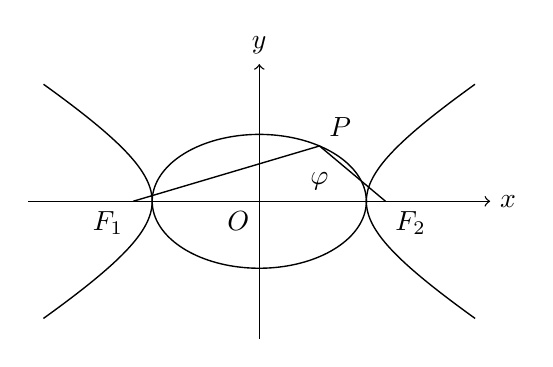
\begin{tikzpicture}[line width=.5pt,x=.85cm,y=.85cm]
  \pgfmathsetmacro{\a}{1.6}
  \pgfmathsetmacro{\f}{sqrt(\a*\a+1)}
  \pgfmathsetmacro{\px}{.9}
  \pgfmathsetmacro{\py}{sqrt(1-(\px/\a)*(\px/\a))}
  \coordinate (O) at (0,0);
  \coordinate (F1) at (-\f,0);
  \coordinate (F2) at (\f,0);
  \coordinate (A1) at (-\a,0);
  \coordinate (A2) at (\a,0);
  \coordinate (P) at (\px,\py);
  \coordinate (H) at (\px,0);
  \draw[->] (-3.45,0)--(3.45,0) node[right] {$x$};
  \draw[->] (0,-2.05)--(0,2.05) node[above] {$y$};
  \draw[domain=0:360,samples=150,smooth]
    plot ({\a*cos(\x)},{sin(\x)});
  \draw[domain=-1.75:1.75,samples=100,smooth]
    plot ({\a*sqrt(1+\x*\x)},\x);
  \draw[domain=-1.75:1.75,samples=100,smooth]
    plot ({-\a*sqrt(1+\x*\x)},\x);
  \draw (F1)--(P)--(F2);
  \node[below left] at (O) {$O$};
  \node[below left] at (F1) {$F_1$};
  \node[below right] at (F2) {$F_2$};
  \node[above right] at (P) {$P$};
  \node[below=6pt] at (P) {$\varphi$};
\end{tikzpicture}
\end{center}
\nopagebreak[4]
\Needspace{4\baselineskip}
\textbf{解析}

\Needspace{5\baselineskip}
（1）双曲线 $\dfrac{x^2}{a^2}-y^2=1$ 的半焦距为

\nopagebreak[4]
\[
c=\sqrt{a^2+1},
\]

\Needspace{5\baselineskip}
故

\nopagebreak[4]
\[
F_1\left(-\sqrt{a^2+1},0\right),\qquad
F_2\left(\sqrt{a^2+1},0\right).
\]

\Needspace{5\baselineskip}
设 $P(x_0,y_0)$ 在椭圆 $\dfrac{x^2}{a^2}+y^2=1$ 上，且不与长轴端点重合。由对称性，不妨设 $0<y_0\le1$。作 $PH\perp F_1F_2$，垂足为 $H$，记

\nopagebreak[4]
\[
\alpha=\angle F_1PH,\qquad \beta=\angle HPF_2,
\]

\Needspace{5\baselineskip}
则 $\varphi=\alpha+\beta$。于是

\nopagebreak[4]
\[
\operatorname{tg}\alpha=\frac{x_0+\sqrt{a^2+1}}{y_0},
\qquad
\operatorname{tg}\beta=\frac{\sqrt{a^2+1}-x_0}{y_0}.
\]

\Needspace{5\baselineskip}
由正切加法公式，

\nopagebreak[4]
\[
\begin{aligned}
\operatorname{tg}\varphi
&=\frac{\operatorname{tg}\alpha+\operatorname{tg}\beta}
{1-\operatorname{tg}\alpha\operatorname{tg}\beta}\\
&=\frac{\frac{2\sqrt{a^2+1}}{y_0}}
{1-\frac{(x_0+\sqrt{a^2+1})(\sqrt{a^2+1}-x_0)}{y_0^2}}\\
&=\frac{2\sqrt{a^2+1}\,y_0}
{x_0^2+y_0^2-(a^2+1)}.
\end{aligned}
\]

\Needspace{5\baselineskip}
因 $P$ 在椭圆上，

\nopagebreak[4]
\[
x_0^2=a^2(1-y_0^2),
\]

\Needspace{5\baselineskip}
代入上式得

\nopagebreak[4]
\[
\operatorname{tg}\varphi
=\frac{2\sqrt{a^2+1}\,y_0}
{a^2(1-y_0^2)+y_0^2-a^2-1}
=-\frac{2\sqrt{a^2+1}\,y_0}
{(a^2-1)y_0^2+1}.
\]

\Needspace{5\baselineskip}
（2）因 $a\ge\sqrt2$，故 $a^2-1\ge1$，分母为正，从而 $\operatorname{tg}\varphi<0$。又 $\varphi\in(0,\pi)$，故

\nopagebreak[4]
\[
\frac{\pi}{2}<\varphi<\pi.
\]

\Needspace{5\baselineskip}
令 $\psi=\pi-\varphi$，则 $0<\psi<\dfrac{\pi}{2}$，且

\nopagebreak[4]
\[
\operatorname{tg}\psi=-\operatorname{tg}\varphi
=\frac{2\sqrt{a^2+1}\,y_0}{(a^2-1)y_0^2+1}
=\frac{2\sqrt{a^2+1}}
{(a^2-1)y_0+\frac{1}{y_0}}.
\]

\Needspace{5\baselineskip}
由均值不等式，

\nopagebreak[4]
\[
(a^2-1)y_0+\frac{1}{y_0}\ge2\sqrt{a^2-1},
\]

\Needspace{5\baselineskip}
故

\nopagebreak[4]
\[
\operatorname{tg}\psi\le
\frac{\sqrt{a^2+1}}{\sqrt{a^2-1}}
=\sqrt{\frac{a^2+1}{a^2-1}}.
\]

\Needspace{5\baselineskip}
等号当且仅当

\nopagebreak[4]
\[
(a^2-1)y_0=\frac{1}{y_0},
\]

\Needspace{5\baselineskip}
即

\nopagebreak[4]
\[
y_0=\frac{1}{\sqrt{a^2-1}}\le1
\]

\Needspace{5\baselineskip}
时成立。由于正切函数在 $\left(0,\dfrac{\pi}{2}\right)$ 内递增，

\nopagebreak[4]
\[
\psi\le\operatorname{arctg}\sqrt{\frac{a^2+1}{a^2-1}},
\]

\Needspace{5\baselineskip}
从而

\nopagebreak[4]
\[
\varphi\ge\pi-\operatorname{arctg}\sqrt{\frac{a^2+1}{a^2-1}}.
\]

\Needspace{5\baselineskip}
因此 $\varphi$ 的最小值为

\nopagebreak[4]
\[
\varphi_0=\pi-\operatorname{arctg}\sqrt{\frac{a^2+1}{a^2-1}}.
\]

\Needspace{5\baselineskip}
（3）将 $\varphi_0$ 改写为

\nopagebreak[4]
\[
\varphi_0=\pi-\operatorname{arctg}\sqrt{1+\frac{2}{a^2-1}}.
\]

\Needspace{5\baselineskip}
由 $\sqrt2\le a\le\sqrt3$ 得

\nopagebreak[4]
\[
2\le a^2\le3,\qquad 1\le a^2-1\le2,
\]

\Needspace{5\baselineskip}
故

\nopagebreak[4]
\[
1\le\frac{2}{a^2-1}\le2,
\qquad
2\le1+\frac{2}{a^2-1}\le3,
\]

\Needspace{5\baselineskip}
从而

\nopagebreak[4]
\[
\sqrt2\le\sqrt{1+\frac{2}{a^2-1}}\le\sqrt3.
\]

\Needspace{5\baselineskip}
由反正切函数的单调性，

\nopagebreak[4]
\[
\operatorname{arctg}\sqrt2
\le\operatorname{arctg}\sqrt{1+\frac{2}{a^2-1}}
\le\operatorname{arctg}\sqrt3=\frac{\pi}{3}.
\]

\Needspace{5\baselineskip}
于是

\nopagebreak[4]
\[
\frac{2\pi}{3}\le\varphi_0\le\pi-\operatorname{arctg}\sqrt2.
\]

\Needspace{5\baselineskip}
即 $\varphi_0$ 的取值范围为

\nopagebreak[4]
\[
\left[\frac{2\pi}{3},\ \pi-\operatorname{arctg}\sqrt2\right].
\]

\gkanswer{答案：（1）$\operatorname{tg}\varphi=-\dfrac{2\sqrt{a^2+1}\,y_0}{(a^2-1)y_0^2+1}$（$y_0$ 为点 $P$ 的纵坐标）；（2）$\varphi_0=\pi-\operatorname{arctg}\sqrt{\dfrac{a^2+1}{a^2-1}}$；（3）$\dfrac{2\pi}{3}\le\varphi_0\le\pi-\operatorname{arctg}\sqrt2$。}

\end{answer}